\section{Introduction} \label{introduction}

The implications of quantum technology for information security attracts a lot of attention in the popular press. But reading headline articles one could be forgiven for taking away something to the effect of,
\begin{quote}
	``Quantum computers will break all our present-day encryption, but quantum cryptography will save the day.''
\end{quote}
Both of these statements are false and there is far more nuance to the intersection between quantum technology and information security than what is often captured in the mainstream media. Here we'd like to give a more detailed overview of what this intersection looks like and how, in our minds, things are likely to play out.

We'll approach this by looking at both classical and quantum cryptographic protocols, their various nuances and caveats, what their different vulnerabilities are, and what implications this has both presently and in the future.

\subsection{What is security?} \label{what-is-security}

When cryptographers talk about security there are different standards of security they have in mind:
\begin{itemize}
	\item \emph{Computational security} is security based on the assumption that adversaries do not possess sufficient computational power to crack our encryption and haven't made any major algorithmic developments that might reduce the computational power they need.
	\item \emph{Information-theoretic security} refers to the situation where a cryptographic system can be mathematically proven to offer perfect security in the absence of any assumptions about computational power.
\end{itemize}

The second standard sets a much higher bar than the former. But because this bar is so high it is often not possible to find cryptographic systems that have this property. When we hear in the media how quantum computers have the potential to break certain cryptographic codes, this is because those codes have relied on the computational security assumption which would not hold were quantum computers available.

If a protocol can be proven to be information-theoretically secure, we're in business and have little to worry about. However very few protocols exhibit this property, and in the classical case, there is only one known example, the one-time-pad, or Vernam cipher (Sec.~\ref{one-time-pad-encryption}), which has extremely limited utility.

In the case of computational security, things are more nuanced, since there are different types of physically realisable computers: quantum and classical. To consider this more rigorously we need to turn to the field of \emph{computational complexity theory} \cite{bib:arora2009computational}, which studies what classes of problems can be solved by different computational models, giving rise to \emph{complexity classes}. There are countless such complexity classes \cite{bib:ComplexityZoo}. Some of these correspond to physically realisable computational models, while others are not physically realisable but useful mathematical tools for use in derivations and proofs. Here we will focus on just a few of these:
\begin{itemize}
	\item \textbf{P} denotes the class of problems that can be solved in polynomial time (as a function of problem size) on a classical computer. These problems are regarded as \emph{classically efficient} by computer scientists.
	\item \textbf{BPP} is the same as \textbf{P} but the computer has access to a random number generator and is able to operate probabilistically. It is known that $\mathbf{P}\subseteq\mathbf{BPP}$ but unproven whether $\mathbf{P}=\mathbf{BPP}$.
	\item \textbf{NP} denotes the class of problems that can be verified (but not necessarily solved) in polynomial time on a classical computer. It is known that \mbox{$\mathbf{P}\subseteq\mathbf{NP}$} and believed but not proven that \mbox{$\mathbf{P}\subset\mathbf{NP}$}. %Whether \mbox{$\mathbf{P}=\mathbf{NP}$} is one of the great open problems in computer science.
	\item \textbf{BQP} denotes the class of problems that can be solved on a quantum computer in polynomial time (i.e efficient for quantum computers). It is known that \mbox{$\mathbf{BPP}\subseteq\mathbf{BQP}$} and believed but not proven that \mbox{$\mathbf{BPP}\subset\mathbf{BQP}$}. If the latter were not the case, there would be no exponential advantage offered by quantum computers over classical ones.
	\item Everything outside \textbf{BPP} and \textbf{BQP} cannot be efficiently solved on any physically realisable computational device (assuming there aren't any laws of physics beyond quantum physics, which is also just a strongly held assumption). \textbf{NP} is an example of a complexity class not believed to be physically realisable.
\end{itemize}

Fig.~\ref{fig:complexity} illustrates the believed relationships between these classes as a Venn diagram, also showing where some classes of cryptographic algorithms belong.

\begin{figure}[!htb]
	\centering
	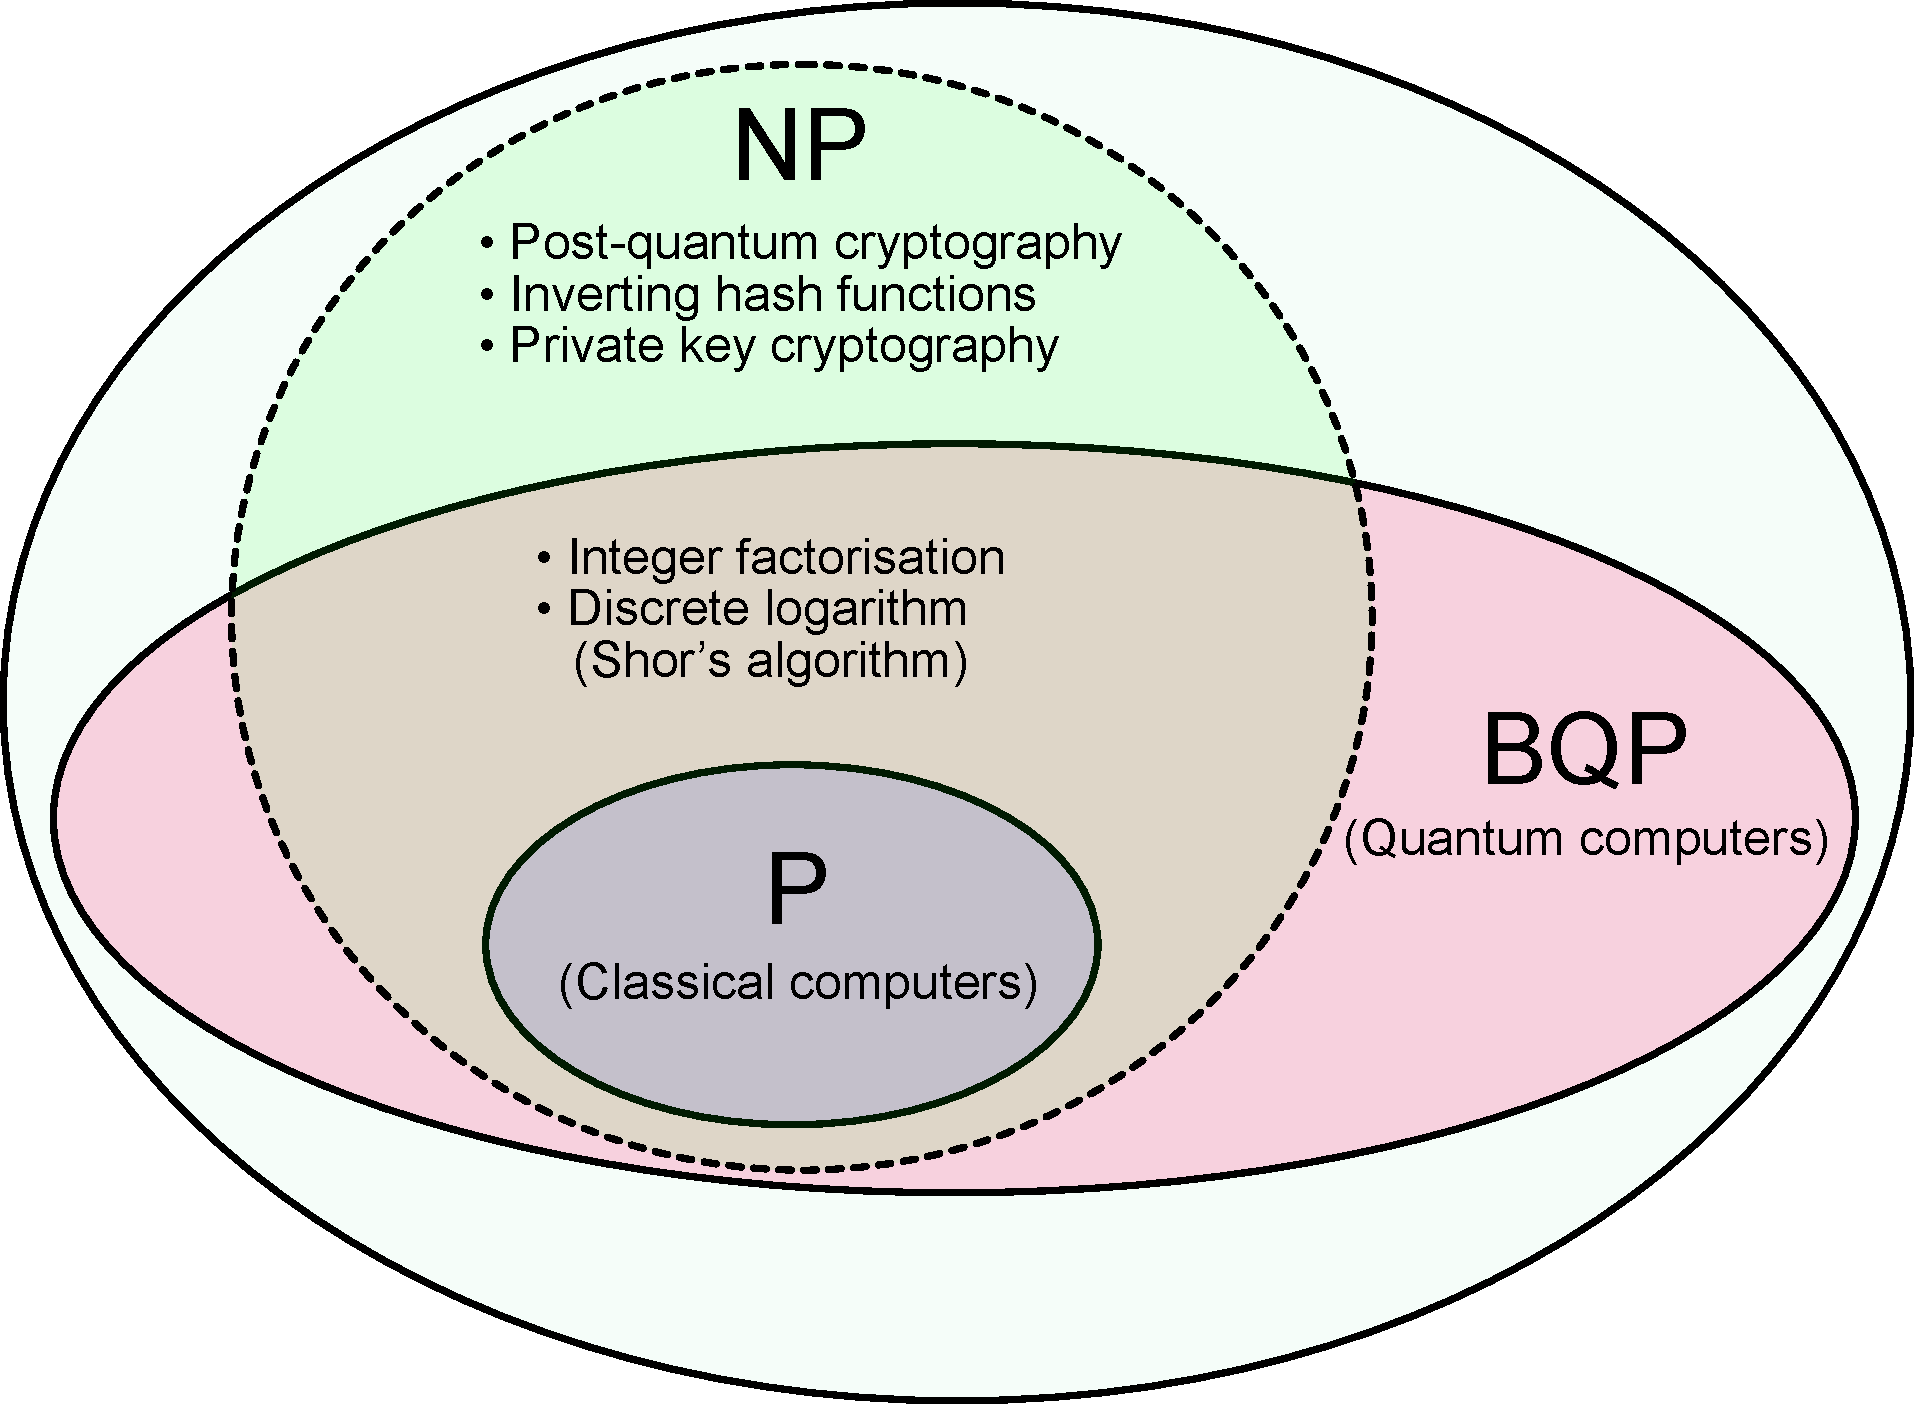
\includegraphics[width=\columnwidth]{figures/Complexity_classes}
	\caption{Venn diagram of the believed relationships between some complexity classes relevant to classical and quantum computing and cryptography. \textbf{P} is the class of problems that can be efficiently solved on a classical computer. \textbf{BQP} is the same for quantum computers. Problems outside \textbf{P} and \textbf{BQP} cannot be efficiently solved by any physically realisable computer (unless the laws of quantum physics are incorrect). Since $\mathbf{P}\subseteq\mathbf{BQP}$, quantum computers can efficiently solve classical problems, but the converse is not believed to be true since it is believed but not proven that $\mathbf{P}\subset\mathbf{BQP}$. \textbf{NP} is the class of problems that can be efficiently verified (as opposed to solved) on a classical computer. While \textbf{P} and \textbf{BQP} are physically realisable computational models, \textbf{NP} is not believed to be, instead being a theoretical one. In general, breaking crypto-systems resides in \textbf{NP} since this can be efficiently verified but not efficiently solved.} \label{fig:complexity}
\end{figure}

If a cryptographic problem is known to reside in \textbf{BQP} but not in \textbf{P}, it can be compromised by quantum computers but not by classical computers. This is where we believe the integer factorisation and discrete logarithm problems reside, which form the basis of current public-key cryptography. Note that neither of these problems has been \emph{proven} to lie outside of \textbf{P} --- it is a strongly held belief based on the fact that these problems have been incredibly well studied. But who knows, perhaps we just haven't studied them hard enough?

For \emph{post-quantum cryptography} (Sec.~\ref{post-quantum-cryptography-pqc}) the ultimate goal is to develop protocols whereby decryption in the absence of knowing the key provably lies outside of \textbf{BQP}. However the field of computational complexity is an extremely challenging one, and many very basic identities are assumed to hold, but not proven to. The most famous example of this is the \textbf{P} versus \textbf{NP} problem, a thorn in the side of computer scientists for decades. Roughly speaking, this statement asks ``if a problem is easy to verify is it easy to solve?'', the answer to which is understood but not proven to be ``no''. The difficulty in proving these complexity relationships often means we have to accept weaker computational security assumptions.